\hypertarget{in-the-beginning}{%
\chapter{In the beginning}\label{in-the-beginning}}

\hypertarget{markdown-philosophy}{%
\section{Markdown philosophy}\label{markdown-philosophy}}

This\paragraphnumber{[1.1]} directory is a skeleton to write a monograph
for \href{https://langsci-press.org}{\emph{Language Science Press}
(LSP)} in Markdown.
\href{https://daringfireball.net/projects/markdown/}{\textsc{markdown}}
was introduced by John Gruber as a easy-to-use method to write content
for webpages. The principles have spread widely and are formally
codified as \href{https://commonmark.org}{\textsc{commonmark}}. The
basic idea is to make it easy to write content, while the details of the
formatting are added by an automatic conversion.

This\paragraphnumber{[1.2]} possibilities of this automatic conversion
has been greatly extended by \href{https://pandoc.org}{\textsc{pandoc}}
as introduced and maintained by John MacFarlane. Pandoc can convert
between dozens of different output formats, allowing for a great freedom
for the visual display of your text. Pandoc also offers many extensions
to the rather basic possibilities of the original markdown/commonmark
proposals. Pandoc also has a robust system to add functionality through
additional modules (called `filters') when needed.

Although\paragraphnumber{[1.3]} Pandoc offers a wide range of
bidirectional conversions between all kinds of formats, the current
system for LSP suggests that you write in Pandoc-enhanced Markdown and
convert from that basis to any desired output format. The problem is
that every format (e.g.~LaTeX, docx, odf) has its own design-quircks,
and Pandoc will never be able to convert every detail between all
formats. The Pandoc-Markdown structure offers a convenient set of markup
options that are garantueed to be converted well and are sufficient for
scientific texts.

Any\paragraphnumber{[1.4]} writer's desire that is currently missing in
Pandoc-Markdown can be easily added by
\href{https://pandoc.org/lua-filters.html}{\textsc{filters}}. In
essence, Pandoc filters are very similar to packages in LaTeX. Because
Pandoc is still relatively new, there are not as many filters available
as there are LaTeX-packages, and there is also not yet a central
repository for filters like \href{https://ctan.org}{\textsc{ctan}} for
LaTeX. However, filters (especially Lua-based filters) are really easy
to write and adapt, especially when compared to the rather arcane format
of LaTeX-packages. The current LSPmarkdown skeleton includes various
special filters to prepare a scientific book that is published on the
open web. Some more details about the rationale for these filters is
explained \href{https://cysouw.github.io/openwebpublishing/}{here}.

There\paragraphnumber{[1.5]} are some major benifits when using
Pandoc-markdown:

\begin{itemize}
\tightlist
\item
  the raw text that you will write is very simple structured and easy to
  read in its raw form, especially when compared to LaTeX.
\item
  markdown strictly follows the design philosophy of separating
  presentation from content. You write the content, while leaving the
  presentation to the output format by an automatic conversion.
\item
  the raw markdown can be converted into many different output formats
  using \href{https;//pandoc.org}{Pandoc}, e.g.~Latex, PDF, HTML, docx,
  etc. Because the output is generated automatically, the styling and
  formatting is always consistent.
\end{itemize}

There\paragraphnumber{[1.6]} are various limitations to the current
markdown setup:

\begin{itemize}
\tightlist
\item
  If you depend on specific functionality provided by LaTeX-packages
  (e.g.~producing syntactic trees), then you can still use them within
  markdown. However, such LaTeX-specific insertions can only be
  conversted to LaTeX and will not be converted to other formats, like
  HTML or docx.
\item
  You are currently restricted to the possibilities as described in
  Sec­tion~\ref{sec:writing}. Anything outside of those bounds have to be
  added by tailor-made Pandoc filters. Suggestions and request for new
  filters are welcome.
\end{itemize}

Note\paragraphnumber{[1.7]} that there are various other approaches that
are similary to the current LSPmarkdown skeleton. Most prominently there
is \href{https://rmarkdown.rstudio.com}{Rmarkdown} and the related
\href{https://bookdown.org}{Bookdown}, which are both based on
\href{https://cran.r-project.org/web/packages/knitr/index.html}{\texttt{knitr}}
by Yihui Xie. Those approaches embed Pandoc inside R-packages and
thereby offer many nice options for the visualisation of quantitative
data. However, these approaches are strongly geared towards usage within
\href{https://posit.co/products/open-source/rstudio/}{RStudio}.

\hypertarget{sec:installation}{%
\section{Installation}\label{sec:installation}}

For\paragraphnumber{[1.8]} writing a book with the LSPmarkdown skeleton
you can use any text editor of you choice. However, prefereably stay
clear of full-fledged word-processors like Microsoft Word or OpenOffice
because they tend to automatically add all kind of markup in the
background, often onbenowst to the user.

Currently,\paragraphnumber{[1.9]} the free editor
\href{https://code.visualstudio.com}{\textsc{visual studio code}} is in
very active development and probably the best choice if you are not yet
entangled to any other text editor. However, any text editor is fine,
e.g.~TextMate, BBedit, Sublime Text, Atom, or even Emacs/vim if you are
so inclined.

In\paragraphnumber{[1.10]} all modern editors (like Visual Studio Code)
it is possible to open a complete directory/folder, so it becomes easy
to switch between editing the different files in the LSPmarkdown
directory. The current LSPmarkdown directory should be the starting
point of your book. Simply rename the directory to your liking and
change the current content (which is only included as an example).

If\paragraphnumber{[1.11]} you want to convert your text to any of the
LSP-based outputs you will need to install some additional software.
This can be done through a package manager like
\href{https://brew.sh}{\texttt{Homebrew}} for macOS. However, it might
be easiest for new users to simple install the following pieces of
software separately:

\begin{itemize}
\tightlist
\item
  \textbf{Pandoc}, install instructions at
  \url{https://pandoc.org/installing.html}
\item
  \textbf{pandoc-crossref}, install instructions at
  \url{https://github.com/lierdakil/pandoc-crossref}. This is a
  Pandoc-filter for cross-referencing that you will have to install
  separately, because depending on your computer you will have to
  install a different version.
\item
  \textbf{LaTeX}, install instructions at
  \url{https://www.latex-project.org/get/}. LaTeX is needed to produce
  PDF output as used at the \emph{Language Science Press}. Included in
  this skeleton is also an option for a quick PDF creation that can be
  used for the preparation of drafts in PDF form.
\item
  \textbf{Libertinus font} from
  \url{https://github.com/alerque/libertinus/releases}. This font is
  used to produce output in the format of the \emph{Language Science
  Press}. The HTML file will attempt to download this font by itself
  when it is not installed on your computer.
\end{itemize}

\hypertarget{setup}{%
\section{Setup}\label{setup}}

To\paragraphnumber{[1.12]} prepare your book there are three basic files
with settings that you will have to adapt to your needs:

\begin{itemize}
\tightlist
\item
  the file \texttt{1\_TITLEPAGE.yaml} contains the basic metadata that
  will end up on your title page
\item
  the file \texttt{2\_CONTENTS.yaml} contains the list of the Markdown
  files that make up your book. Simply list the filenames in the order
  as they should occur in the book here.
\item
  the file \texttt{3\_SETTINGS.yaml} contains a few further
  user-settings. Specifically, you will have to specify the location of
  your bibliography here (see also Sec­tion~\ref{sec:references}).
\end{itemize}

The\paragraphnumber{[1.13]} current LSPmarkdown directory is prepared
for direct upload as a git-repository, e.g.~at Github or Gitlab. That is
probably the easiest way to share your work with others, also in any
pre-publication status. There are a few files included here for a more
transparent sharing of your work online:

\begin{itemize}
\tightlist
\item
  a \texttt{LICENSE} file with a
  \href{https://creativecommons.org/licenses/by/4.0/}{\textsc{cc-by}}
  license in accordance to the LSP guidelines.
\item
  a \texttt{README.md} file. Please write a few lines in this
  \texttt{README} file to introduce your book.
\item
  a \texttt{NEWS.md} file. This file can initally be ignored because it
  is geared to documenting updates for possible subsequent editions of
  the book.
\end{itemize}

\hypertarget{sec:writing}{%
\chapter{Writing in Pandoc-markdown}\label{sec:writing}}

\hypertarget{basic-editing}{%
\section{Basic editing}\label{basic-editing}}

The\paragraphnumber{[2.1]} basic principles of writing in Markdown are
explained at various places online. However, the most authorative
summary is provided by the
\href{https://commonmark.org}{\textsc{commonmark}} project. The most
basic rules are:

\begin{itemize}
\tightlist
\item
  use hashes (\#) at the start of a line for headings. The number of
  hashes indicates the heading level.
\item
  use stars (*) around text that should be set in \emph{italics}.
\item
  square brackets \texttt{{[}{]}} are used for all kind of links and
  cross-references (see below).
\end{itemize}

\hypertarget{pandoc-advanced-editing}{%
\section{Pandoc advanced editing}\label{pandoc-advanced-editing}}

The\paragraphnumber{[2.2]} possibilities of markdown are enhanced by
Pandoc with various crucial formatting options as specified in the
\href{https://pandoc.org/MANUAL.html\#pandocs-markdown}{\textsc{pandoc
user's guide}}. These formatting options will all be retained in the
various conversions from Markdown into other formats (e.g.~HTML or PDF).
For example, \href{https://pandoc.org/MANUAL.html\#footnotes}{footnotes}
are included by using the following format inside your text at the
position where the footnote mark should occur.\footnote{This is an
  example footnote. Footnote text between square brackets and a
  circumflex symbol before the brackets.}

\begin{verbatim}
^[Footnote text between square brackets and a circumflex symbol before the brackets.]
\end{verbatim}

In\paragraphnumber{[2.3]} the current LSPmarkdown framework there is an
additional filter added that will change strikethrough formatting (by
enclosing double tildes) into \textsc{small caps} formatting. This is a
convenience option because linguistic texts often use small caps, but
only rarely strikethrough. To remove this automatic conversion, simply
remove the filter \texttt{strikeout-to-smallcaps} from the conversion
files (e.g.~from the file \texttt{tohtml.yaml}).

\hypertarget{cross-referencing}{%
\section{Cross-referencing}\label{cross-referencing}}

Pandoc\paragraphnumber{[2.4]} itself contains some basic
cross-referencing options. However, it is strongly recommended to
install the extra software
\href{https://github.com/lierdakil/pandoc-crossref}{\textsc{pandoc-crossref}}.
This allows for various flexible options to automatically insert
internal cross-references in your text. Basically, you add a label to a
heading by adding it behind the heading like this:

\begin{verbatim}
## Some Heading {#mylabel}
\end{verbatim}

In\paragraphnumber{[2.5]} your text you then refer to this heading by
typing \texttt{{[}@mylabel{]}} which will result in a cross reference
like this: Sec­tion~\ref{sec:writing}. \textsc{pandoc-crossref} has many
more possibilities and options as explained in detail in the
\href{https://lierdakil.github.io/pandoc-crossref/}{user's guide}.

\hypertarget{linguistic-examples}{%
\section{Linguistic examples}\label{linguistic-examples}}

To\paragraphnumber{[2.6]} add linguistic examples, the LSPmarkdown
skeleton includes a Pandoc-filter
\href{https://github.com/cysouw/pandoc-ling}{\textsc{pandoc-ling}}. A
full \href{https://cysouw.github.io/pandoc-ling/readme.html}{user's
guide} describing all options and limitations is available. Basically,
you can add linguistic examples using the following format:

\begin{verbatim}
::: ex
a. This is an example sentence.
b. And another one.
:::
\end{verbatim}

This\paragraphnumber{[2.7]} will result in a numbered example as shown
below. You can refer to this example using abbreviations like
\texttt{{[}@next{]}} before the examples or \texttt{{[}@last{]}} after
the example, e.g.~see example (\ref{ex2.1}).

\begin{samepage}
\ea \judgewidth{} \label{ex2.1} 
  \ea [] { This is an example sentence. }
  \ex [] { And another one. }
  \z
\z
\end{samepage}

\hypertarget{figures}{%
\section{Figures}\label{figures}}

To\paragraphnumber{[2.8]} insert figures into your text, prepare figures
separately and store them in the directory \texttt{figures}. In your
markdown then add a line like the following below the table. This will
be automatically numbered, and you can use the code
\texttt{{[}@fig:crossreferencelabel{]}} in your text to refer to the
figure, for example Figure~\ref{fig:crossreferencelabel}.

\begin{verbatim}
![Caption text here](figures/myfigure){#fig:crossreferencelabel}
\end{verbatim}

To\paragraphnumber{[2.9]} prepare HTML output it is prefereable to
convert any figure into
\href{https://en.wikipedia.org/wiki/SVG}{\textsc{svg}} format. There are
many \href{https://convertio.co/pdf-svg/}{online converters} that can do
this. You can include different file formats with the same filename into
the directory \texttt{figures}, e.g.~\texttt{myfigure.pdf} and
\texttt{myfigure.svg}.

\begin{figure}
\hypertarget{fig:crossreferencelabel}{%
\centering
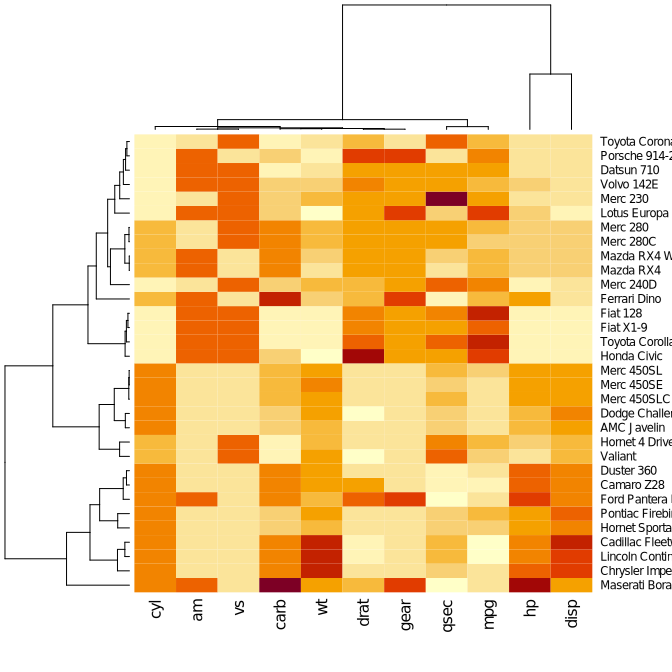
\includegraphics{figures/myfigure.pdf}
\caption{This is an example figure.}\label{fig:crossreferencelabel}
}
\end{figure}

\hypertarget{tables}{%
\section{Tables}\label{tables}}

The\paragraphnumber{[2.10]} situation to include tables is not yet very
user friendly in Pandoc-Markdown. The editing and conversion of tables
is currently a field of active development within Pandoc, so this will
probably be improved substantially in the near future. For now, check
out the possibilities for formatting tables in the Pandoc
\href{https://pandoc.org/MANUAL.html\#tables}{user's guide}. If you use
Visual Studio Code, then there is a useful extension that might be
helpful for formatting tables called
\href{https://marketplace.visualstudio.com/items?itemName=shuworks.vscode-table-formatter}{\textsc{table
formatter}}.

\hypertarget{tbl:crossreferencelabel}{}
\begin{longtable}[]{@{}rllc@{}}
\caption{\label{tbl:crossreferencelabel}This is an example
table}\tabularnewline
\toprule\noalign{}
Right & Left & Default & Center \\
\midrule\noalign{}
\endfirsthead
\toprule\noalign{}
Right & Left & Default & Center \\
\midrule\noalign{}
\endhead
\bottomrule\noalign{}
\endlastfoot
12 & 12 & 12 & 12 \\
123 & 123 & 123 & 123 \\
1 & 1 & 1 & 1 \\
\end{longtable}

To\paragraphnumber{[2.11]} add a caption to the table, add a line like
the following below the table. This will be automatically numbered, and
you can use the code \texttt{{[}@tbl:crossreferencelabel{]}} in your
text to refer to the table, for example see
Table~\ref{tbl:crossreferencelabel}.

\begin{verbatim}
Table: Caption text here {#tbl:crossreferencelabel}
\end{verbatim}

\hypertarget{sec:references}{%
\section{References}\label{sec:references}}

Pandoc\paragraphnumber{[2.12]} includes a
\href{https://pandoc.org/MANUAL.html\#citations}{\textsc{citeproc}}
extension to treat references and bibliography using the
\href{https://citationstyles.org}{\textsc{citation style language
(csl)}} framework. The current framework uses the
\href{https://www.zotero.org/styles?q=linguistics}{`unified style sheet
for linguistics'} by default. There are various ways to include
references, but two options seem to be most useful:

\begin{itemize}
\tightlist
\item
  if you manage your references in
  \href{http://www.bibtex.org}{\textsc{bibtex}} style, then you only
  have to add a path to your BibTeX-file in \texttt{3\_SETTINGS.yaml}
\item
  if you manage your references with
  \href{https://www.zotero.org}{Zotero} then you should additionally
  install
  \href{https://retorque.re/zotero-better-bibtex/installation/}{BetterBibTeX}.
\end{itemize}

For\paragraphnumber{[2.13]} the Zotero/BetterBibTeX workflow, you will
have to additionally do the following:

\begin{itemize}
\tightlist
\item
  create an synchronised BibTeX file in Zotero by using
  \texttt{File\ \textgreater{}\textgreater{}\ Export\ Library…} checking
  \texttt{keep\ updated}. Save this file somewhere where you can easily
  find it on your computer. The simplest solution would be save this
  file inside the LSPmarkdown directory.
\item
  add a path to this file in \texttt{3\_SETTINGS.yaml}.
\item
  set
  \texttt{Preferences\ \textgreater{}\textgreater{}\ Better\ BibTeX\ \textgreater{}\textgreater{}\ Automatic\ export\ \textgreater{}\textgreater{}\ Automatic\ export:\ On\ change}.
\end{itemize}

In\paragraphnumber{[2.14]} both options your references will have a
`citation key' which typically uses a format like \texttt{chomsky1957}
(but this format can be changed to your liking). To include a reference
in your text use the link as shown below. This will result in a
reference in your text (\protect\hyperlink{ref-Chomsky1957}{Chomsky
1957}: 23). You can add anything you like after the citations key,
typically page numbers. To suppress the name inside the brackets, add a
dash-minus symbol before the `@' symbol. This will result in a reference
to Bloomfield (\protect\hyperlink{ref-Bloomfield1925}{1925}).

\begin{verbatim}
[@Chomsky1957: 23]
[-@Bloomfield1925]
\end{verbatim}

\hypertarget{making-the-book}{%
\chapter{Making the book}\label{making-the-book}}

A\paragraphnumber{[3.1]} few different settings-files are included in
this LSPmarkdown skeleton to prepare the final book from your markdown
source. These are \texttt{yaml}-files with various settings. Such files
are called \texttt{defaults-files} in pandoc-parlance (see the
\href{https://pandoc.org/MANUAL.html\#defaults-files}{pandoc
documentation}).

\begin{itemize}
\tightlist
\item
  the file \texttt{tohtml.yaml} is used to convert to LSP-styled HTML
\item
  the file \texttt{topdf.yaml} is used to convert to a quick-and-easy
  draft PDF
\item
  the file \texttt{totex.yaml} is used to convert to LSP-styled LaTeX
  and subsequent LSP-styled PDF
\end{itemize}

To\paragraphnumber{[3.2]} use these default-files you will have to open
a terminal/shell in the current directory. If you use Visual Studio Code
and you have opened the whole LSPmarkdown directory with
\texttt{File\ \textgreater{}\textgreater{}\ Open\ Folder…} then this is
really easy, also when you have never used a terminal/shell. Simply open
a terminal/shell through the menu
\texttt{Terminal\ \textgreater{}\textgreater{}\ New\ Terminal} and then
type the command as specified below.

\hypertarget{lsp-style-html}{%
\section{LSP-style HTML}\label{lsp-style-html}}

To\paragraphnumber{[3.3]} convert your markdown to HTML type the
following command in your terminal and hit return:

\begin{verbatim}
pandoc -d tohtml.yaml
\end{verbatim}

As\paragraphnumber{[3.4]} a result there will be a new file called
\texttt{index.html} in the directory \texttt{docs} with the final HTML
output. This file is completely self-contained and does not need any
other files to work properly. You can immediately open this file locally
from you computer by double-clicking it. It will open locally in you
default web browser.

Because\paragraphnumber{[3.5]} this file is completely self-contained
you can easily share it with other people (just send them the file).
When you sync your whole directory with GitHub you can immediately
publish this file using
\href{https://docs.github.com/en/pages/getting-started-with-github-pages/configuring-a-publishing-source-for-your-github-pages-site}{\texttt{GitHub\ Pages}}.
Note that the fonts used in the LSP style are Libertinus Serif (for the
main text) and Arimo (for the title page). When these fonts are not
installed on your computer the browser will attempt to fetch them from
the internet.

For\paragraphnumber{[3.6]} final LSP-publication there are few
additional minor tweaks to be made:

\begin{itemize}
\tightlist
\item
  The copyright info has to be added at the start of the HTML file. This
  information has to be manually changed in the file
  \texttt{settings/LSP-copyright.md}. To include this file in the final
  output open the defaults-file \texttt{tohtml.yaml} and add the line as
  explained there.
\item
  You might want to remove the coloured hypelinks by deleting the
  respective lines at the bottom of the settings-file
  \texttt{3\_SETTINGS.yaml}.
\item
  To add colour to the title page, you will have the change to colour in
  the file \texttt{settings/LSP-css.yaml} in the line
  \texttt{background-color}.
\end{itemize}

\hypertarget{draft-pdf}{%
\section{Draft PDF}\label{draft-pdf}}

To\paragraphnumber{[3.7]} convert your markdown to PDF you can use the
following command in the terminal:

\begin{verbatim}
pandoc -d topdf.yaml
\end{verbatim}

This\paragraphnumber{[3.8]} will produce a PDF-file called
\texttt{book.pdf} in the directory \texttt{docs}. This PDF does not use
the LSP styling. Instead, the PDF will use the default LaTeX-style from
the conversion-software Pandoc. The advantage of this option is that
this conversion to PDF is much quicker and easier than the complete LSP
pathway as described below. This is particularly useful if you want to
produce a quick PDF version for printing or reviewing of your text. Note
that you will need LaTeX to be installed on your computer, see
Sec­tion~\ref{sec:installation}

\hypertarget{lsp-style-pdf}{%
\section{LSP-style PDF}\label{lsp-style-pdf}}

Finally,\paragraphnumber{[3.9]} there is a conversion option to prepare
your book for LaTex-based LSP publication. The preparation of a final
book for LSP is somewhat more involved because there are various checks
and additional fine-tuning needed for a polished real-life publication.
Basically the procedure is as follows: first, convert your markdown into
raw LaTex, and second, use this LaTex to proceed through the regular LSP
pipeline. To convert you markdown to raw LaTeX you can use the following
command in your terminal:

\begin{verbatim}
pandoc -d totex.yaml
\end{verbatim}

This\paragraphnumber{[3.10]} will produce a tex-file called
\texttt{all.tex} in the directory \texttt{latex/chapters}. The directory
\texttt{latex} is a slightly adapted version of the default LSP skeleton
to produce a book. You will have to make a few more changes in this
directory to produce a complete LSP book:

\begin{itemize}
\tightlist
\item
  add author and title information in the file
  \texttt{latex/localmetadata.tex}.
\item
  add any figures (preferably in PDF format) into the directory
  \texttt{latex/figures}
\end{itemize}

Then\paragraphnumber{[3.11]} you can produce a draft version of the
final LSP styled PDF by typing the following command in your terminal:

\begin{verbatim}
make -C latex
\end{verbatim}

This\paragraphnumber{[3.12]} will take some time, and might very well
spit out many TeX-errors. For now simply ignore these messages. If this
process gets stuck, type ``x'' to break and ask somebody for help. If it
finishes, then there will a PDF-file called \texttt{main.pdf} in the
directory \texttt{latex} with your LSP-styled book. The final tweaks to
this process will be performed together with the people from the
\emph{Language Science Press}.

\hypertarget{bibliography}{%
\chapter*{Bibliography}\label{bibliography}}
\addcontentsline{toc}{chapter}{Bibliography}

\markboth{Bibliography}{}
\markright{Bibliography}{}

\hypertarget{refs}{}
\begin{CSLReferences}{1}{0}
\leavevmode\vadjust pre{\hypertarget{ref-Bloomfield1925}{}}%
Bloomfield, Leonard. 1925. On the sound-system of central {Algonquian}.
\emph{Language} 1(4). 130--156.

\leavevmode\vadjust pre{\hypertarget{ref-Chomsky1957}{}}%
Chomsky, Noam. 1957. \emph{Syntactic structures}. The Hague: Mouton.

\end{CSLReferences}
